\section{Classical Collective Intelligence}
In 1990s, John Smith wrote a book called Collective Intelligence in Computer-Based Collaboration which is now considered the classical Collective Intelligence. The book has two main parts: one is the foundation concepts about collective intelligence and its theoretical origin; the other one is about the core ideas in the theory \cite{cibook}. Smith regards collaboration as an information processing activity and computer system as a part of this collaboration system together with human. And key elements in the system that across both computer system and human are Collective Memory, Collective Processing, Collective Strategy and Collective Awareness and Control.

\subsection{Collaboration as an Information Processing Activity}
The work of a group is focused in the production of some concrete product or in problem-solving. Although groups differ significantly in their sies, location, duration, completion of the group mission and the ways the group works, there are surprisingly siginificant similarities among their distributed activities. So as a group, they share a body of knowledge about their work. The ways to share knowledge among group members across time and location, and how to use the knowledge to guide their practices into achieving the goals are the two main questions to look in the theory. In order to find the similarities, Simith examined into different collaboration scenarios to illustrate the range of behaviors commonly found in the collaborative groups, and to describe the informaiton flow from one to another. In summary, groups are all concerned with producing some type of tangible product. All of them produced several types of intangible knowledge, some shared within the group and some kept private. For all the tangible, ingangible and ephemeral konwledge that have been created in the process, they transfer from one form to another form among the group members. Please refer to the figure below.

\begin{figure}[!h]
\centering
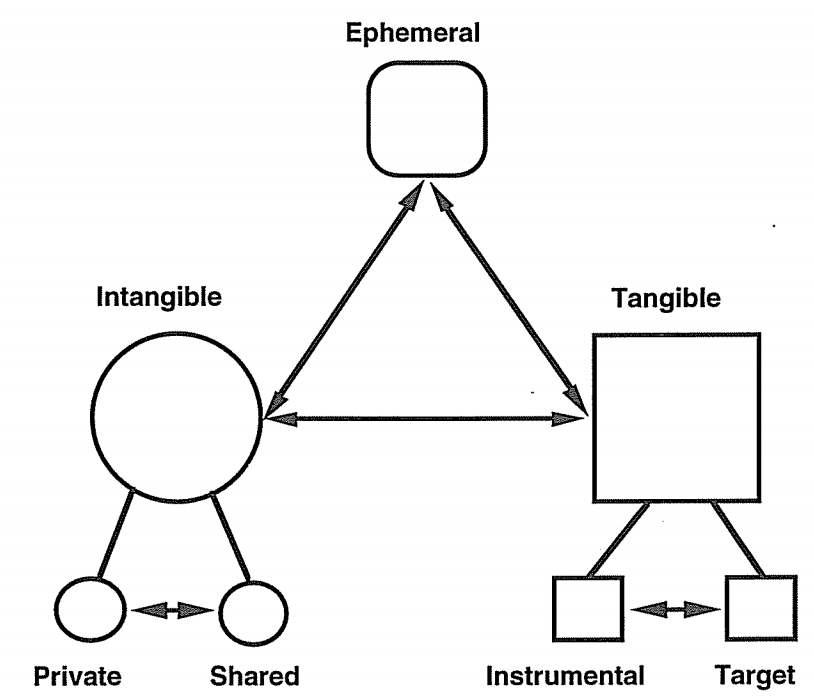
\includegraphics[width=0.9\columnwidth]{figure/IPS}
\caption{Information Types in a Collaboration System}
\label{fig:IPS}
\end{figure}

\subsection{Computer Support for Collaboration}
Collaborative group work requires a variety of tools to facilitate the process. This work focused on computers as the tool to help create knowledge, tranform knowledge and enhance the information flow among different members in the group. In addition to computers, the author also looked into various collabroative softwares - both synchronous and asynchronous - in the support of independent work and collaborative work. Some asychronous tools include email, FTP, Network File Systems and so on. Synchronous tools like audio/video conferencing was also examined in the work. Smith also proposed a comprehensive system for collaboration, showed in the following figure. Three workstations are connected to a hypermedia storage system and to one another by a high-speed network. The same conferenced brower can be seen on each workstation, with supporting video window. 

\begin{figure}[!h]
\centering
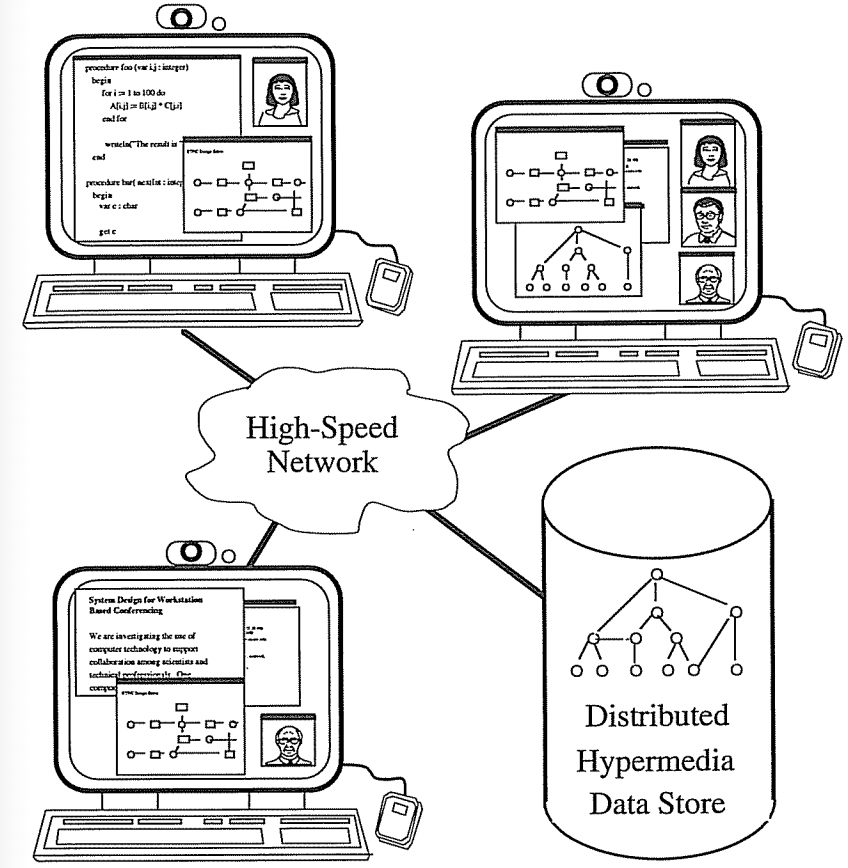
\includegraphics[width=0.9\columnwidth]{figure/ABC}
\caption{Artifact-Based Collaboration System}
\label{fig:ABC}
\end{figure}

\subsection{Concepts of Collective Intelligence}
There are four identified in the collective intelligence system shared with human and computer: collective memory, processing, strategy and awareness/control.

\subsubsection{Collective Memory}
In this collaborative system, memory systems provide the storage of both long-term and short-term memories. Additionally to the storage, the constructs that function as a form of collective memory for the group is also examined. It includes provisions for the long-term storage and retrieval of information, analogous to human long-term memory, and it provides contexts in which that information can be activated and processed, analogous to working memory. 

\subsubsection{Collective Processing}
Collective processing focuses on the form and function of individual small-grained processes that operate in the contexts identified as the group's working memory. They are responsible for basic actions such as retrieving and defining concepts, identifying relationships, building conceptual structures, making changes to those structures and storing results. In this way, it enables the group to function as an information processing system and reach the goal of the group.

\subsubsection{Collective Strategy}
Strategy, on the other hand, extends its scope beyond individually independent entities and processing and considers the relation between one and another. The focus is on the patterns in the sequences of processes that occur in the behavior of a group. By engaging processes not as isolated actions but in coherent sequences, groups are able to function in purposeful ways and to accomplish goals.

\subsubsection{Awareness and Control}
The work talks about two metacognitive issues - awareness and control. Awareness plays a large role in enabling an individual to produce intellectual products that are coherent and internally consistent. It also examines the ways in which a group can piece together partial, but overlapping bodies of knowledge among its members to produce partial but overlapping fields of awareness.

Authority and administrative control wihtin groups in relation to issues of self-controal in individuals are also important part of the discussion. A balance between delegated and centralized authority is needed to motivate groups and to enable them to produce work with intellectual integrity.
























